\section{Рабочий проект}
\subsection{Классы, используемые при разработке сайта}

Можно выделить следующий список классов и их методов, использованных при разработке web-приложения (таблица \ref{class:table}).

\renewcommand{\arraystretch}{0.8} % уменьшение расстояний до сетки таблицы
\begin{xltabular}{\textwidth}{|X|p{2.5cm}|>{\setlength{\baselineskip}{0.7\baselineskip}}p{4.85cm}|>{\setlength{\baselineskip}{0.7\baselineskip}}p{4.85cm}|}
\caption{Описание классов, используемых в приложении\label{class:table}}\\
\hline \centrow \setlength{\baselineskip}{0.7\baselineskip} Название класса & \centrow \setlength{\baselineskip}{0.7\baselineskip} Модуль, к которому относится класс & \centrow Описание класса & \centrow Методы \\
\hline \centrow 1 & \centrow 2 & \centrow 3 & \centrow 4\\ \hline
\endfirsthead
\caption*{Продолжение таблицы \ref{class:table}}\\
\hline \centrow 1 & \centrow 2 & \centrow 3 & \centrow 4\\ \hline
\finishhead
HomeView & Главный модуль & HomeViev – Класс представляет собой представление главной страницы. & def get(self, environ) Метод обрабатывает GET-запросы к главной странице.
Выводит заголовок страницы\\
\hline ContactUsView & Главный модуль & ContactUsView – Класс представляет собой представление страницы " О нас ". & def get(self, environ) Метод обрабатывает GET-запросы к странице " О нас ".
\hline CheckoutView & Главный модуль & CheckoutView – Класс представляет собой представление страницы оформления заказа. & def get(self, environ) Метод обрабатывает GET-запросы к странице оформления заказа.
\hline ProductView & Главный модуль & ProductView – Класс представляет собой представление страницы продукта. & def get(self, environ) Метод обрабатывает GET-запросы к странице продукта.
\hline View & Главный модуль & View – Базовый класс для представлений веб-страниц. & def get(self, environ) Абстрактный метод для обработки GET-запросов.
\end{xltabular}

\renewcommand{\arraystretch}{1.0} % восстановление сетки


\subsection{Системное тестирование разработанного web-сайта}

На рисунке \ref{main:Главная} представлена главная страница сайта онлайн магазина кроссовок.

\begin{figure}[H] % H - рисунок обязательно здесь, или переносится, оставляя пустоту
\center{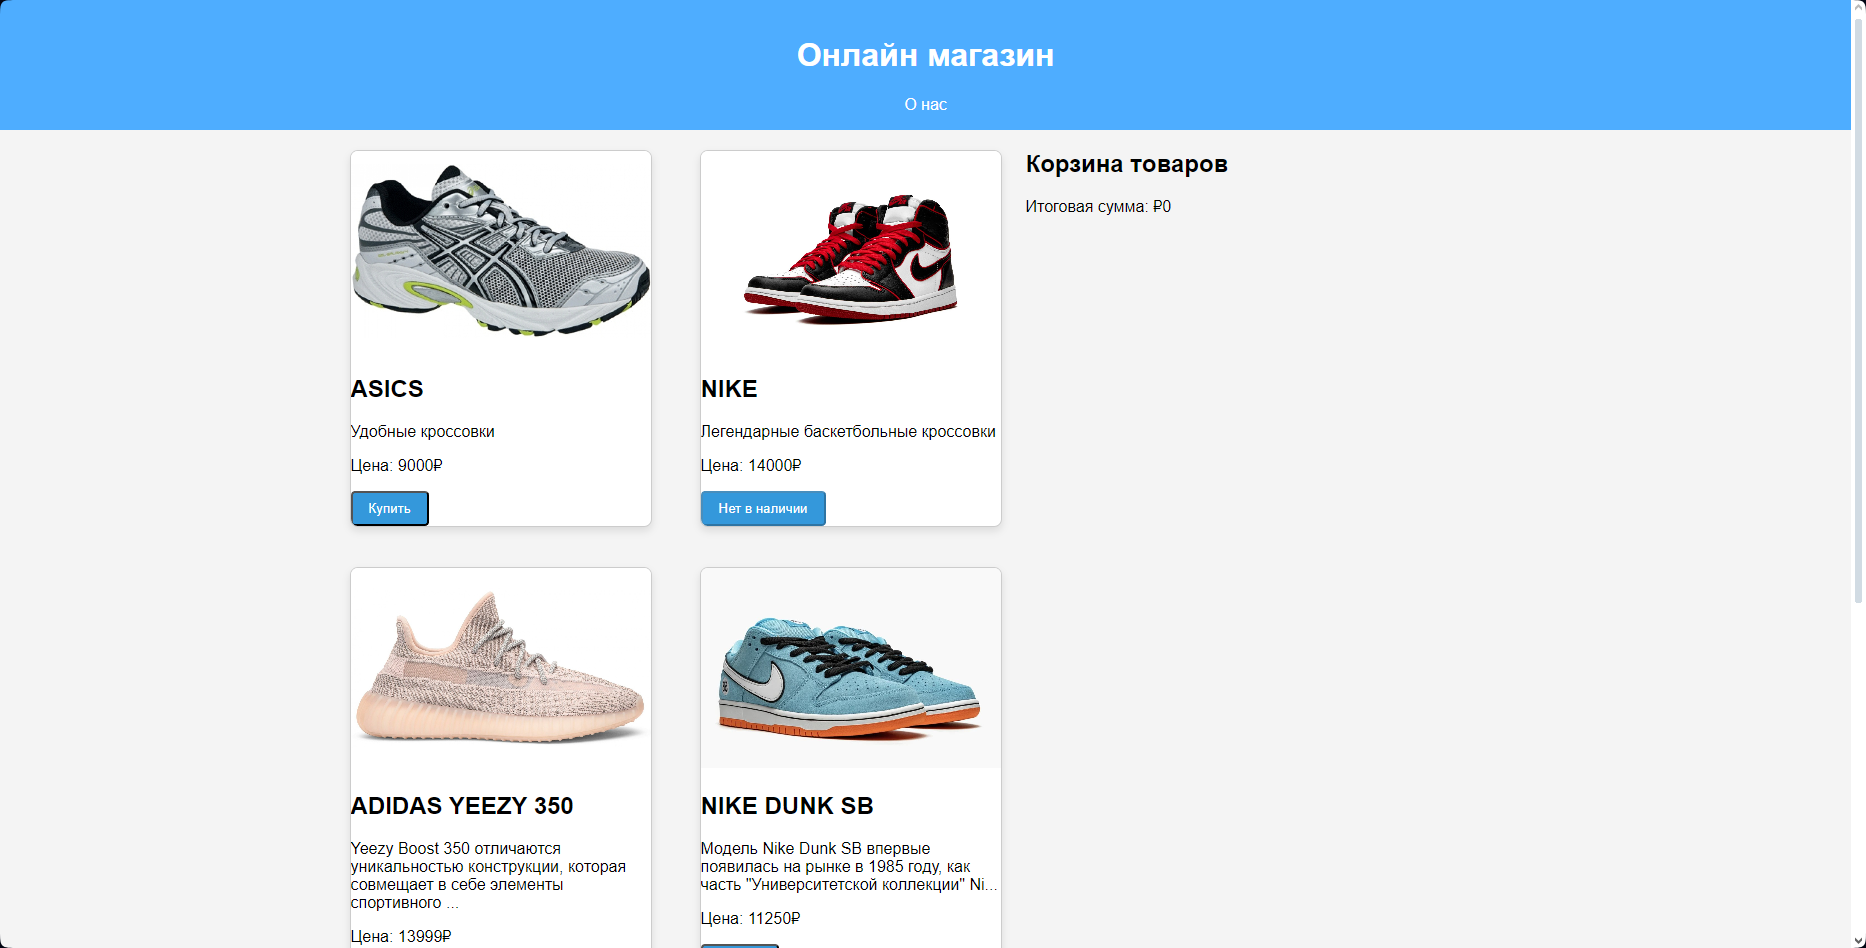
\includegraphics[width=1\linewidth]{Главная}}
\caption{Главная страница сайта онлайн магазина кроссовок}
\label{main:Главная}
\end{figure}


На рисунке \ref{menu:Вывод} представлен динамический вывод товара при нажатии на картинку.
\begin{figure}[ht]
\center{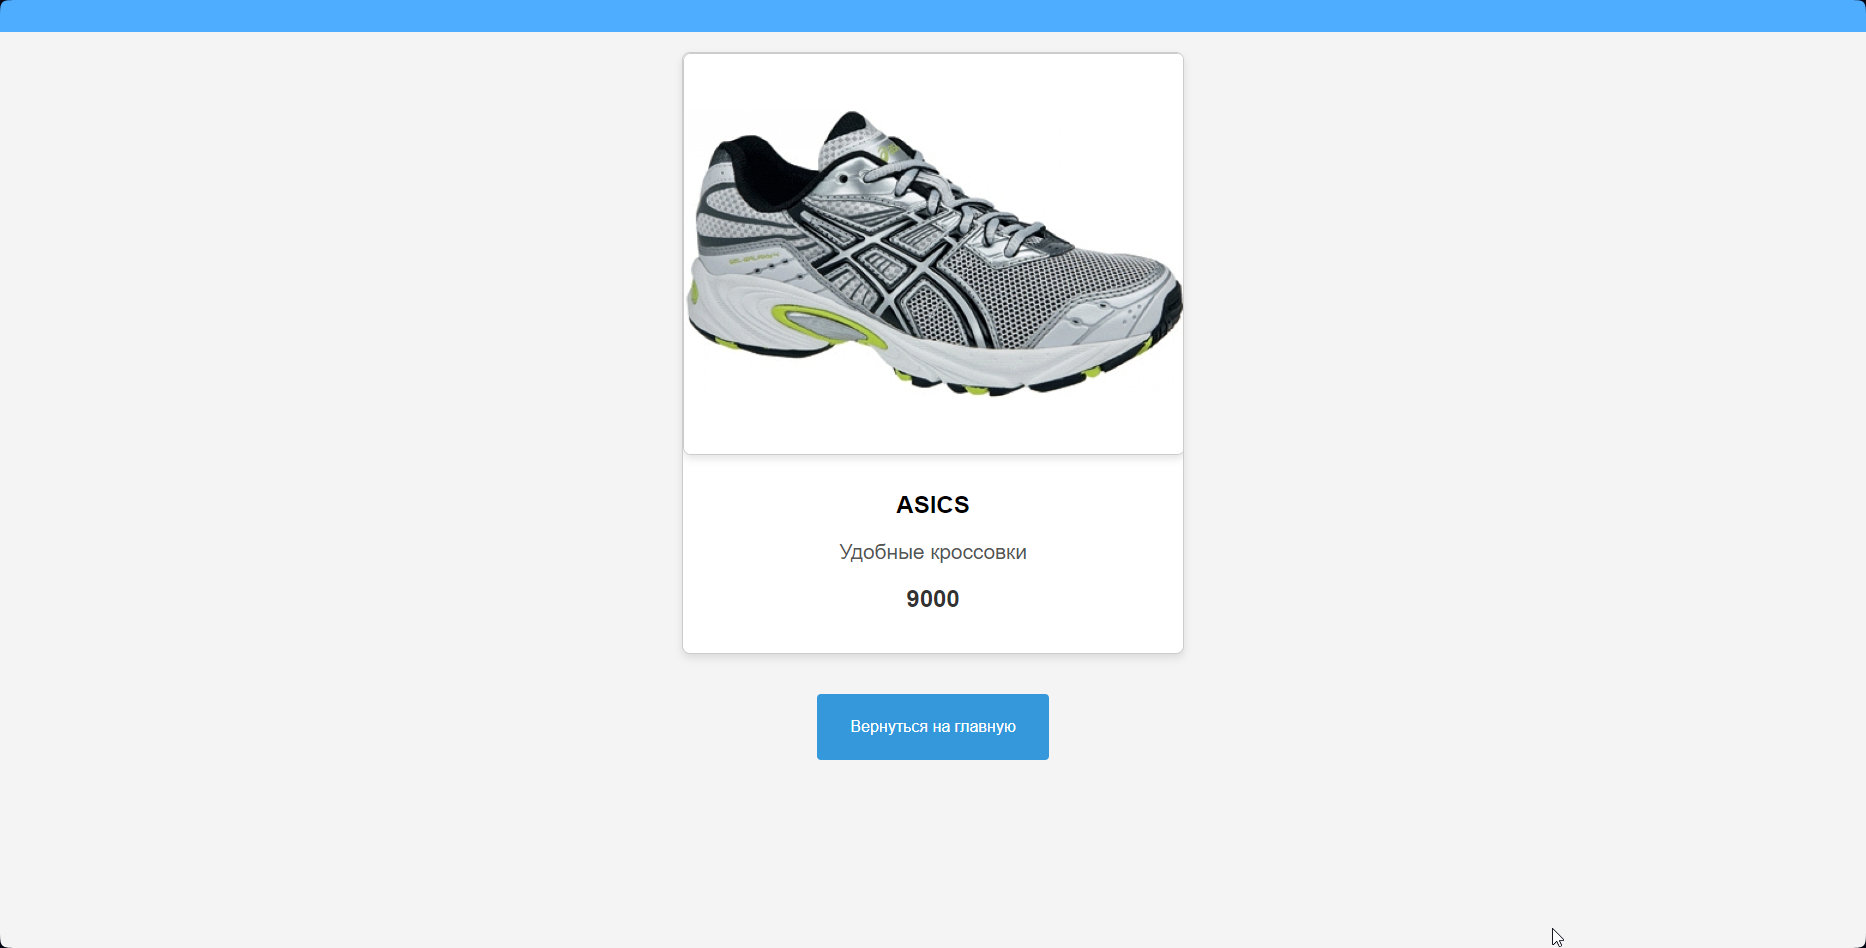
\includegraphics[width=1\linewidth]{Вывод}}
\caption{Динамический вывод товара}
\label{menu:Вывод}
\end{figure}

\newpage
На рисунке \ref{enter:Заказ} представлена страница оформления заказа.
\begin{figure}[ht]
\center{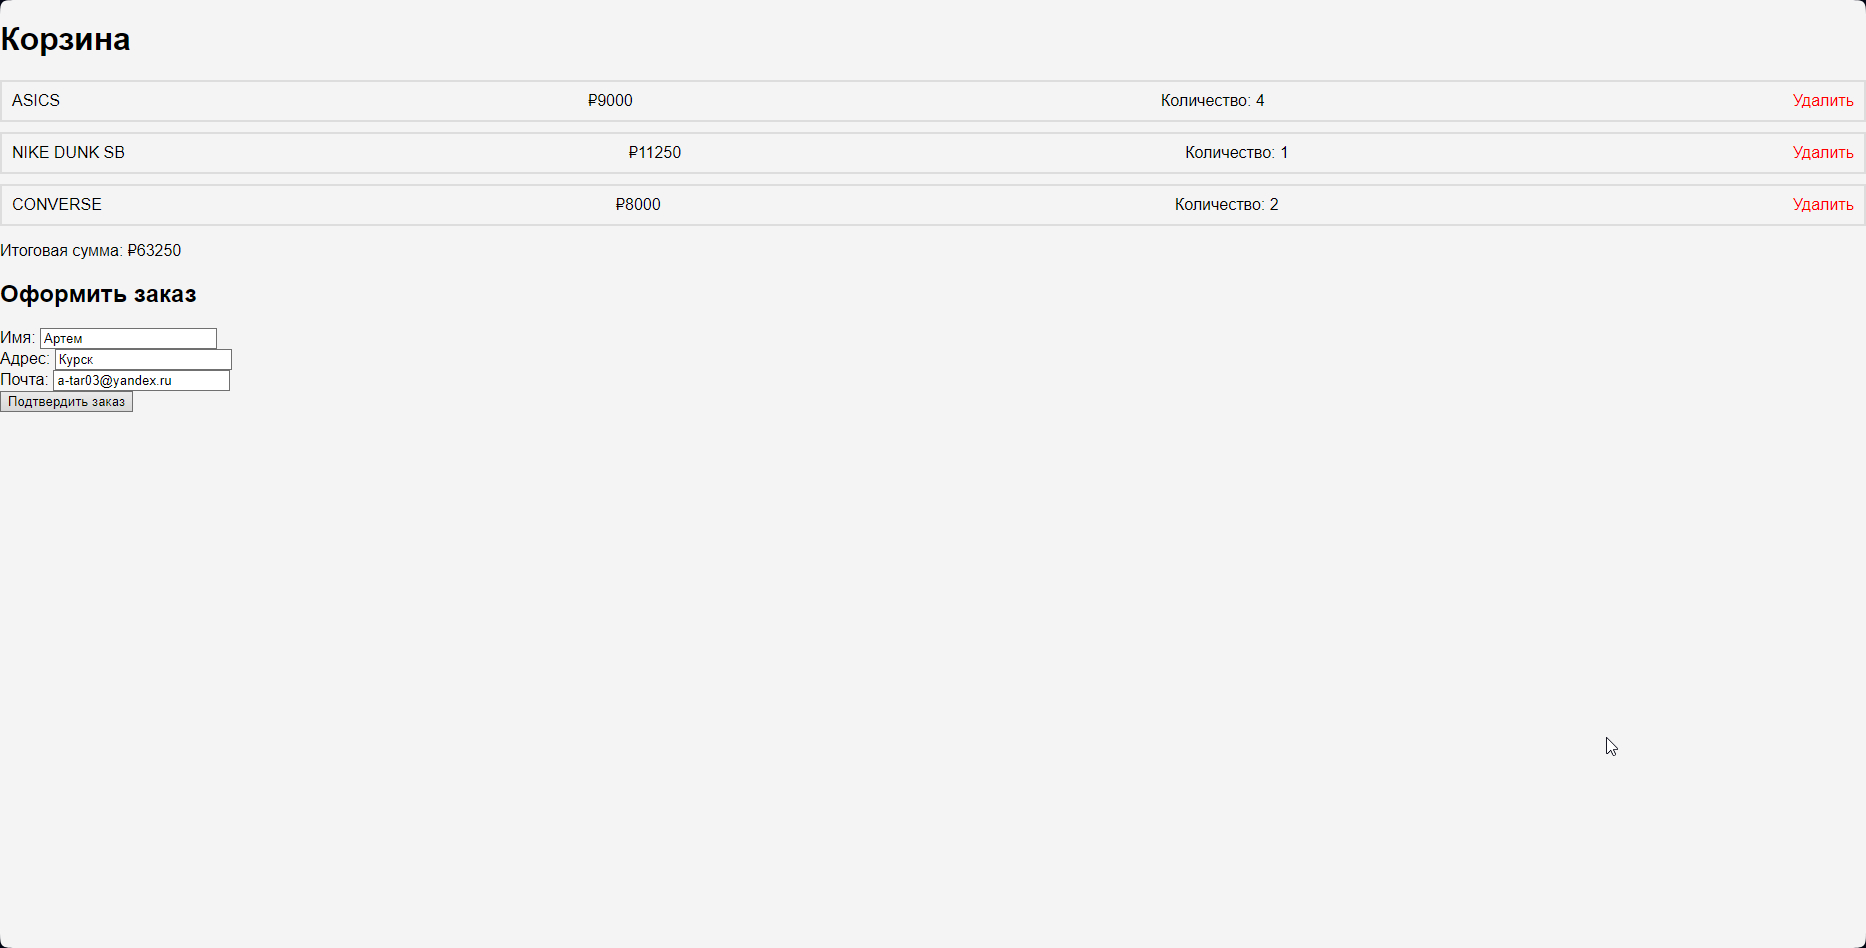
\includegraphics[width=1\linewidth]{Заказ}}
\caption{Страница оформления заказа}
\label{enter:Заказ}
\end{figure}

